\chapter{Problem Statement}
\label{cha:PS}
\section{Mathematics Background}
\label{sec:MB}
The medium between the transmitting antenna of the sender and the receiving antenna of the receiver is generally called "channel". The characteristics of wireless signal changes as it travels from the sender to the receiver. These characteristics depend upon the distance between the two antennas, the paths taken by the signal, the existence of line of sight (LoS) paths between the two stations or the reflection, refraction and diffraction of the signal due to some objects in the paths. \\
In general, the power profile of the received signal can be obtained by convolving the power profile of the transmitted signal with the impulse response of the channel. Convolution in time domain is
equivalent to multiplication in the frequency domain. Therefore, the transmitted signal \textit{x}, after propagation through the channel \textit{H} becomes \textit{y}:
\begin{gather}
    y(f) = H(f)*x(f)+n(f)
\end{gather}

\textit{H(f)} is the channel response, and \textit{n(f)} is the noise. All the variable are all functions of the signal frequency \textit{f}.
The key components of the channel response are \textit{path loss}, \textit{shadowing} and \textit{multipath}.\vskip 1em
The simplest channel is the free space line of sight channel without objects between the receiver and
the transmitter or around the path between them. A convenient way to express the Free Space Path Loss is in terms of dB is:
\begin{gather}
    \text{FSPL}(\text{dB}) = 20\log\left(d\right) + 20\log\left(f\right)+ 20\log\left(\frac{4 \pi}{c}\right)
\label{eq:1}
\end{gather}
where:
\begin{itemize}
    \item $f$ is the signal frequency in \SI{}{\Hz};
    \item $d$ is the distance from the transmitter in \SI{}{\m};
    \item $c$ is the speed of light in \SI{}{\meter\per\second};
\end{itemize}\vskip 1em
If there are any objects along the path of the signal, some part of the transmitted signal is lost. This effect is called \textit{shadowing}. With shadowing the path loss becomes:
\begin{gather}
    \text{FSPL}(\text{dB}) = 20\log\left(d\right) + 20\log\left(f\right)+ 20\log\left(\frac{4 \pi}{c}\right) + \chi
\label{eq:2}
\end{gather}
Here $\chi$ is a normally distributed random variable which represent the effect of shadowing. As a result of shadowing, power received at the points that are at
the same distance d from the transmitter may be different and have a lognormal distribution. This
phenomenon is referred to as \textbf{lognormal shadowing}.\vskip 1em
The objects located in the environment of the wireless signal can reflect the signal. Some reflected waves are also received at the receiver. These reflected signals take different paths, so they arrive at the receiver with different amplitude and phase. These multiple signals can result in increased or decreased received power. \vskip 1em
Channel models can be characterized as deterministic or stochastic. Deterministic models are used for site-specific channel modeling; they consist of an environment model and a wave propagation model. The environment model describes position, geometry, material composition and surface properties of the wave propagation relevant objects and obstacles. The Maxwell equations, form the basis for all investigation of electromagnetic fields. In practical applications an analytic solution of the Maxwell equations it is not possible due to the high computation time. On the other hand, stochastic models can be computationally efficient and through probability distribution taken from statistical analyses of data collected from measurement campaigns, can emulate the main channel effects. \vskip 1em
In the field of stochastic communication channels Markov chains \cite{kemeny1960finite} are a powerful and commonly used tools. They consists of a finite number of states and corresponding state transition probabilities.\\
The Markov chain can be in one state at a time. The transition between states is governed by transition probability and takes place each time a digit is generated. If the state is not directly visible, but the output is visible the model is called \emph{hidden}.\vskip 1em
The availability of efficient algorithms for the extraction of HMM parameters from experimental data makes their application is vehicular communication simple and computationally inexpensive.\\
The use of Hidden Markov Chains in communication channels goes back to the model proposed by Gilbert \cite{gilbert1960capacity} in the 1960s.
\begin{figure} [H]
    \centering
    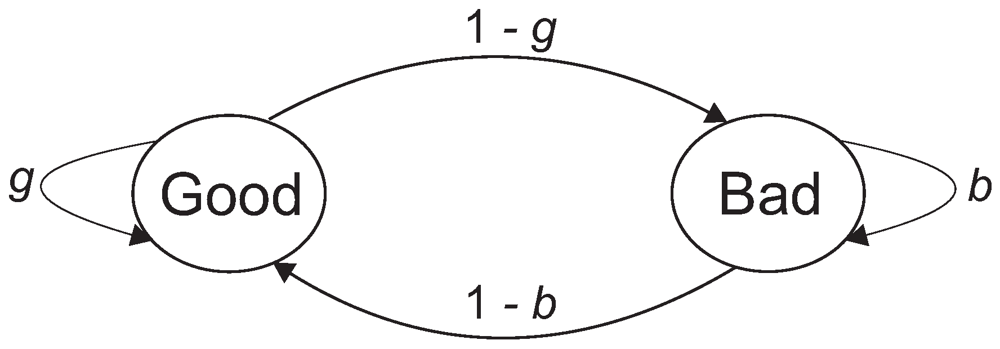
\includegraphics[width=0.5\textwidth]{fig/gilbert.png}
    \caption{The model proposed by Gilbert}
    \label{fig:gil}
\end{figure}
As can be seen in \Cref{fig:gil}, he proposed a chain with two state called \emph{Good} and \emph{Bad}. In the state Good the noise digit is always 0. In the state Bad a coin is tossed to decide whether the digit will be 0 or 1. To simulate burst noise, the states Bad and Good must tend to persist. So the probability of remaining in a state is larger than the probability of changing the state i.e. \textbf{\textit{g}} \textgreater\textgreater \textbf{\textit{1-g}} and \textbf{\textit{b}} \textgreater\textgreater \textbf{\textit{1-b}}. This can be avoided using a Continuous Time Markov Chain for which the time spent in each state is governed by non-negative real values with an exponential distribution.\vskip 1em
When modelling real-world vehicular channels a basic Gilbert's model with constant parameters should not be used, since the performance of the communication links is strongly dependent on the distance between nodes. To maintain an accurate representation of the propagation effects, the author of \cite{shivaldova2013vehicular} proposed to divide the measured error patterns into \emph{N} parts, corresponding to \emph{N} disjoint intervals of the same length. Once the parameters are estimated, they are combined to form a range-dependent Gilbert model, which has the same properties of the original, expect that the model parameters change according to the distance between the two vehicles.
\section{The Veins Framework Stack}
\subsection{Connection Manager}
The role of the \textbf{Connection Manager} module is to manage and coordinate the connections between all nodes. Nodes are connected with each other only when they are within the \textbf{maximal interference distance}. This distance is a bound on the maximal distance at which one nodes can still disturb the communication of a neighbor. To calculate the distance, the Connection Manager needs some parameters which are taken as input from the \textbf{omnetpp.ini} file, these are the max transmission power, the carrier frequency, the Path Loss coefficient and a sensitivity threshold, which is a lower bound on the received power, because a frame can never be decoded if its received power it is smaller than sensitivity threshold. \Cref{tab:param} below shows the parameters and the values used to compute the distance and used in each simulation.
\begin{table}[H]
    \centering
    {\tabulinesep=1.2mm
    \begin{tabu}{l|l}
        \hline
        Parameter & Value  \\
        \hline
        Max Transmission Power (pMax) & \SI{100}{\mW}$\sim$ \SI{20}{\dB}    \\
        Signal attenuation threshold (sat) & \SI{-94}{\dB} \\
        Path Loss coefficient ($\alpha$)  & 2.3 \\
        Carrier frequency (f)& \SI{5.890e+9}{\Hz} \\
        \hline
    \end{tabu}}
    \caption{Connection Manager parameters}
    \label{tab:param}
\end{table}
The module use the formula defined in \cite{sommer2012applicability}, which is derived from the \emph{Free Space path loss} model by introducing an additional environment-dependent path loss exponent $\alpha$, yielding
\begin{gather}
    A = 10\log\left(\left(\frac{4\pi f}{c}\right)^2 d^{\alpha}\right)
\label{eq:10}
\end{gather}
where \emph{d} is equal to the distance between the two antennas and \emph{c} is the speed of light measured in \si{\meter\per\second}. To compute the distance the equation has to be solved in the \emph{d} variable, yielding
\begin{gather}
    \newcommand*\rfrac[2]{{}^{#1}\!/_{#2}}
    d =\left(\frac{c^2 10^{\left(\frac{A}{10}\right)}}{16\pi^2 f^2}\right)^{\alpha^{-1}}
    \label{eq:4}
\end{gather}
using the parameters shown in \Cref{tab:param} and the attenuation $A$ equals to \SI{114}{\dB}, the resulting distance is \SI{751}{\meter}.
This means that in order to communicate, the distance between two vehicles has to be below \SI{751}{\meter}.\\
The Connection Manager will check every time the connections between a given vehicle and its neighbors, if the distance between the vehicle and a neighbor is below the interference distance the vehicles will remain neighbors, otherwise the Connection Manager will disconnect the two vehicles.\vskip 1em
The same thing is done when a new vehicle enter in the scenario, after the registration of the Nic, the Connection Manager will update the neighbors of the vehicle, while when the vehicle exit from the scenario, the Connection Manager will delete the Nic and disconnect the Nic with its old neighbors.
\subsection{Application and Protocol Layer}
In Veins each vehicle is provided with an \textbf{Application Layer} running on the top of the network stack and a \textbf{Protocol Layer} for the dissemination of the messages.
The role of the Application Layer is to load the parameters of the scenario, exchanging data with SUMO through the \textbf{TraCiCommandInterface} in order to dynamically set the parameters of each car or fetching the information of a car to synchronize it with the surrounding vehicles.\vskip 1em
Instead, the role of the Protocol Layer is to implement communication strategy to share information between the vehicles in the scenario, this includes choosing which kind of message has to be exchanged, insert in the messages information about position, speed, destination (manly broadcast) and so on and so forth. Both Application and Protocol Layers come with a basic class that provides primitives to allow an easier implementation of new protocols.
\subsection{Mac Layer}
The \textbf{Mac Layer} in Veins implements the specification described in the IEEE 1609.4 standards, which defines the multi-channel and Quality of Service (QoS) operation of radios, thus vehicles with a single radio will periodically switch between multiple channels.\vskip 1em
While there is only one Control Channel (CCH) to which every radio must tune for \SI{50}{\ms} in every \SI{100}{\ms}, there are others Service Channels (SCHs) on which a radio can transmit and receive in the remaining 50 ms time slots. Furthermore, to counter minor synchronization inexactness and to account for different frequency switching speeds of radios, a \SI{4} {\ms} guard interval at the beginning of every slot is added.\vskip 1em
When the Mac Layer receive a packet from the upper layer, it will assign the packet to one queue based on the channel type and the level of priority specified in the packet. Then a packet can be sent when the exponential back-off counter for its queue is 0 and the physical channel was idle for at least the time of one Arbitration Interframe Space (AIFS) which depends on the priority.\vskip 1em
When the packet is ready to be sent it will be encapsulated in a frame with the MAC address of both sender and receiver. To the frame will be attached also a \textbf{Signal} which stores the physical representation of the signal of an Physical Layer frame, this includes the start, duration and the propagation of the signal, and also the transmission power, bitrate, attenuations caused by effects of the channel on the signal during its transmission and the receiving power.\\
More information about the \textbf{Signal Module} can be found in \cite{kopke2008simulating}, while in \cite{eckhoff2012multichannel} the authors gives a deep prospective of the implementation of the Mac Layer.  \vskip 1em
On receiver side, when the Mac Layer receives a frame that is completely received and not noise from the Physical Layer, it will check the destination address and then send the frame to the upper layer. Also, the Physical Layer can send a control message to the Mac Layer to change the radio state if a transmission is over or changing the channel status to a specific value.
\subsection{Physical Layer}
The \textbf{Physical Layer} is directly connected to the Mac Layer via OMNeT++ channels and is able to send messages to other Physical Layers through sub-classing from \textbf{ChannelAcces}. Apart from message sending ans receiving, this layer acts as an interface between Physical Layer messages called \textbf{AirFrame} and the Analog Model and the Decider which are also initialized by this layer.\\
During the initialization, it will fetch the parameter from the \textbf{omnetpp.ini} and the \textbf{config.xml}, and then initialize the Analog Models and the Decider according to the parameters specified in the configuration files.\vskip 1em
When it receives a message from the upper layer, it will encapsulate the Mac Frame in a AirFrame and then send the frame down to the channel, which will send the frame to all the Nics connected with the sender.\vskip 1em
When receiving a message from the channel, the Physical Layer first passes the frame to the Analog Model and then it passes the message twice to the Decider, the first time at the beginning of the message and then at the end of the message. Once the decider has computed the bit error, the message has to be sent to the Mac Layer.\vskip 1em
Furthermore, the Physical Layer stores all the AirFrame in the \textbf{ChannelInfo} class which provides a function that returns all the AirFrame in the channel in a given intervals. This function is used by the Decider to calculate the Signal to Noise Ratio (SNR) and the Signal to Interference plus Noise Ratio (SINR) of a frame.
At the end, once a frame has been decoded and sent to the Mac Layer, it is deleted from the channel.
\subsection{Analog Model}
An \textbf{Analog Model} is a filter responsible for changing the attenuation value of a Signal. The attenuation of a Signal is calculated by implementations of fading, shadowing and path-loss models. An arbitrary number of analog models can be plugged into the Physical Layer. Each Analog Model is a filter class for Signals. The Analog Models which will be used and their parameters can be specified in the \textbf{config.xml}. Summing up the attenuation of all Analog Models gives the
attenuation part of the signal, which is calculated at the start of the reception of a message. Together with the sending power of a received packet the Decider can then compute the SNR and the SINR and, thus, bit errors.
\subsection{Decider}
The \textbf{Decider} has three main functions. The first time an AirFrame is parsed by the Decider, it will classify that AirFrame as a receivable messages or noise. The receiving power is calculated by multiplying the transmission power with the attenuation of every receiving Analog Model. If that power is under a sensitivity threshold specified in the \textbf{omnetpp.ini} then the frame will be treated as noise and it will not be decoded at its end. Also, a frame will not be decoded if the Nic is currently synced with another frame or the Radio State is in Transmission Mode.\vskip 1em
The latest time that the Decider can request the message from the Physical Layer is at the end of the receiving process of the message. This is also the time when the decider has to calculate the bit errors for the messages that are not treated as noise or interference. Depending on what are specified in the parameters, the Decider can compute both SINR and SNR or just the SINR. Compute both can be useful in order to understand if an error in the header or the payload of the frame is due to the interference of others frames in the channel in that interval or just to a collision, but on the other hand it will increase the computation time and so the simulation time. \vskip 1em
To compute the bit errors, the Decider requests all intersecting frames from the \textbf{ChannelInfo} and than compute the SINR or the SNR for that frame. The last task of the Decider is to provide information about the channel state. The Mac Layer can request the Decider to sense the channel for a certain amount of time. The decider then returns whether the channel is currently idle or busy.
\Cref{fig:scenario} shows an example of a possible scenario. Vehicles are disposed into a highway of four lanes. Vehicle A is sending a message to B with a distance of 20 meters. The neighbors of vehicle B are the vehicles within the circle. When vehicle B receives the frame from A, the Decider will compute the SINR or the SNR using the frames coming from its neighbors.
\begin{figure} [H]
    \centering
    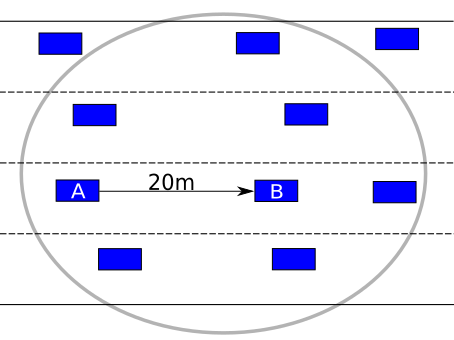
\includegraphics[width=0.6\textwidth]{fig/example.png}
    \caption{An example of scenario}
    \label{fig:scenario}
\end{figure}

\section{Problems and solutions}
\label{sec:prob}
While this approach gives the best results in term of accuracy, it can be really computationally expensive in term of simulation time. For example, thinking about a scenario with 640 vehicles, if each vehicle has more than 90 neighbors and the message propagation is governed by broadcast \textbf{beacons} sent by each vehicle to its neighbors every \SI{0.1}{\second}, in the channel there will be every second at least 500000 frames. This will obviously be extremely expensive due to the fact that to compute the SINR, the Decider will parse each frame in the channel at a given interval. \vskip 1em
To solve this problem, we proposed and implemented a Markov model with the aim to reduce the computation and maintain a good accuracy with respect to the original model. We developed a range and neighbors dependent Markov chain based on the Gilbert model explained in the first section of this chapter. The model is a CTMC, so the transition between the \textbf{Good} and \textbf{Bad} states is governed by two exponential variables whose values indicate the time spent in each state before the next transition.\vskip 1em
The choice of the granularity, i.e., the length of the interval in which the model parameters do not change, and the time spent in each states are essential for the accuracy of our range and neighbors modified Gilbert model. The granularity cannot be chosen arbitrarily small since dividing the measured error pattern into very short intervals will increase the computation of the parameters and there is the possibility that there are not enough data to estimate some intervals. On the other hand, estimating the model parameters for large intervals will inevitably reduce the computation but there is the possibility that the results do not reflect the distribution of the data used for the estimation.\vskip 1em
The data used for the estimation are a user behaviour. He can decide to use data that are taken by real experiment, extrapolating data from previous simulations or use randomly generated data to study the model under certain situations.
\section{Implementation}
\label{sec:implementation}
In order to implement the new model we modified some modules of the Veins Framework.\\
In the \textbf{ConnectionManager} we added the possibility to use a maximal interference distance specified by the user in the \textbf{omnetpp.ini} configuration file. Also we added the possibility to save the results of a simulation in a \textbf{CSV} file specified by the user in the configuration file. By default the file is structured as a tuple with information about the distance between the sender and the receiver, the number of neighbors of the receiver, if a packet has been correctly decoded or not, the IDs of the receiver and the sender and the simulation time of the recording.\vskip 1em
In the \textbf{Signal Module} we added two variable to store information about the distance between two vehicles and the list of neighbors of the receiver. Since this information will not be initialized in the Signal class, we added also four methods to store and fetch the information in a different module.\vskip 1em
In the \textbf{BasePhyLayer} in the \textbf{handleAirFrame} function, we fetched the neighbors of the receiver through the instance of the ConnectionManager and then we set the neighbors in the Signal via the function \textbf{setNeighbors} of the Signal class.\vskip 1em
In the \textbf{PhyLayer80211p} we added the initialization functions of the new Decider and the new Analog Model, also we added the possibility to schedule the recording intervals and a function that wrote the statistics received from the Decider in the csv. Since each vehicle has a own Physical Layer and they will write on the same csv, we decided to initialize the csv in the \textbf{ConnectionManager} which is global to each vehicle.\vskip 1em
The role of the new \textbf{Analog Model}, is to simply compute the distance between the receiver and the sender and then put it in the Signal through the method \textbf{setDistance}. The distance is not computed in the Physical Layer because it is needed only by the new model, so it is better to compute it in a new Module. If user needs the distance in the original model, he can simply add this new Analog Model the ones he is already using.\vskip 1em
The new \textbf{Decider} is the core of the new model. In the \textbf{config.xml} the user can insert the parameters of the Decider, these are: the center frequency of the channel, the intervals and the granularity of the model, the mean of the exponential variables representing the time spent in each state and the file that contains the parameters of the model. \\
Each Decider stores the channel's information between the receiver and the sender in an \textbf{HashMap} structured as follow: \textbf{$\left(\textit{sender\_id},\left(\textit{slotted distance,neighbors,channel state, next transition}\right)\right)$}.\\ When the Decider receives the frame from the Physical Layer for the first time, it will compute the slotted distance and then it will check if an entry with the Id of the sender is already in the map. If the map does not contain the entry, the Decider will add the sender to the map and set the next transition time as the actual simulation time plus the value of the transition from the Good state to the Bad state. \\
At the end of the receiving process of the message the Decider will compute the error rate of the frame. This will be only done if the frame is not under the minimum sensitivity.
If the distance and the neighbors between the two vehicles have been changed with respect to a previous communication between the two vehicles, the probability of being in a state or in another is based on the mean value of being in one of the two state. I.e. if the channel is on state Good at instant \textit{t}, the probability of being in the same state at instant \textit{t+1} is given by:
\begin{gather} \frac{\text{E[Good]}}{\text{E[Good]}+\text{E[Bad]}}
    \label{eq:5}
\end{gather}
while if the distance and the neighbors remain the same it means that the condition of the channel are not changed, and so the Decider will change the state of channel until the time of the next transition is larger than the actual simulation time, the following algorithm shows the computation of the actual state:\vskip 2em
\begin{center}
\begin{algorithm}[H]
    \caption{Compute State}
    $now\gets simTime\left(\right)$\;
    $P\textsubscript{Good}\gets \dfrac{E[Good]}{E[Good]+E[Bad]}$\;
    \eIf{$distance == old\_distance$ {\bf and} $neighbors == old\_neighbors$}
    {\While{$time\_to\_switch < now$}
        {\eIf{$state == Good$}
            {
            $time\_to\_switch \gets time\_to\_switch + \exp\left(\lambda\textsubscript{G}\right)$\;
                $state \gets Bad$\;
            }
            {
            $time\_to\_switch \gets           time\_to\_switch + \exp\left(\lambda\textsubscript{B}\right)$\;
                $state \gets Good$\;

            }
        }
    }
    {\eIf{$uniform\left(0,1\right) < P\textsubscript{Good}$}
        {
           $time\_to\_switch \gets SimTime\left(\right)$\;
            $state \gets Good$\;
        }
        {
            $time\_to\_switch \gets SimTime\left(\right)$\;
            $state \gets Bad$\;
        }
    }
\end{algorithm}
\end{center}\vskip 2em
At the end, the probability of correctly decode a frame is computed and the result is sent to the Physical Layer, which will write the result in the csv and send the frame to the upper layer.
\newpage
